\documentclass[sigconf,nonacm,screen]{acmart}

%% ---------------------------------------------------------------------------
%% CONCLAVE: A Domain-Agnostic Multi-Agent Architecture for
%%           Real-Time Explainable Risk Detection
%% arXiv preprint (cs.CR / cs.LG). Built with acmart sigconf.
%% ---------------------------------------------------------------------------

\usepackage{tikz}
\usetikzlibrary{arrows.meta,positioning,fit,backgrounds,calc,shapes.geometric}
\usepackage{pgfplots}
\pgfplotsset{compat=1.17}
\usepackage{booktabs}
\usepackage{multirow}
\usepackage{listings}
\usepackage{xcolor}

% A breakable underscore/dot for long monospace identifiers
% (events.{domain}.labels, security_lateral_movement) so they wrap inside the
% narrow ACM column instead of overflowing the gutter.
\newcommand{\us}{\_\allowbreak}   % underscore + permitted break
\newcommand{\dt}{.\allowbreak}    % dot + permitted break
% mop up any remaining tight lines rather than overflowing into the gutter
\emergencystretch=2.5em
\hbadness=2500

% Data-driven figures: macros + .dat files emitted by benchmark/make_paper_data.py
% Auto-generated by benchmark/make_paper_data.py — do not edit by hand.
\newcommand{\fraudattackmean}{0.88}
\newcommand{\fraudattacks}{96}
\newcommand{\fraudauc}{0.999}
\newcommand{\fraudblockf}{0.909}
\newcommand{\fraudblockfn}{16}
\newcommand{\fraudblockfp}{0}
\newcommand{\fraudblockfpr}{0.0}
\newcommand{\fraudblockprec}{100.0}
\newcommand{\fraudblockrec}{83.3}
\newcommand{\fraudblocktn}{236}
\newcommand{\fraudblocktp}{80}
\newcommand{\fraudclean}{236}
\newcommand{\fraudcleanmean}{0.16}
\newcommand{\fraudflagfpr}{9.7}
\newcommand{\fraudflagprec}{80.7}
\newcommand{\fraudflagrec}{100.0}
\newcommand{\fraudlatmax}{8997}
\newcommand{\fraudlatpfifty}{1820}
\newcommand{\fraudlatpninefive}{3632}
\newcommand{\fraudlatpninenine}{7940}
\newcommand{\fraudmixallow}{213}
\newcommand{\fraudmixblock}{80}
\newcommand{\fraudmixreview}{39}
\newcommand{\fraudnbustout}{8}
\newcommand{\fraudncardtestingring}{80}
\newcommand{\fraudndec}{332}
\newcommand{\fraudnfraudato}{8}
\newcommand{\fraudponeprec}{98.9}
\newcommand{\fraudponerec}{93.8}
\newcommand{\fraudponethr}{0.55}
\newcommand{\fraudrecbustout}{100}
\newcommand{\fraudreccardtestingring}{100}
\newcommand{\fraudrecfraudato}{100}
\newcommand{\judgeendpoint}{OpenRouter}
\newcommand{\judgemodel}{google/gemini-3.1-flash-lite}
\newcommand{\secattackmean}{0.38}
\newcommand{\secattacks}{36}
\newcommand{\secauc}{0.819}
\newcommand{\secblockf}{0.468}
\newcommand{\secblockfn}{25}
\newcommand{\secblockfp}{0}
\newcommand{\secblockfpr}{0.0}
\newcommand{\secblockprec}{100.0}
\newcommand{\secblockrec}{30.6}
\newcommand{\secblocktn}{218}
\newcommand{\secblocktp}{11}
\newcommand{\secclean}{218}
\newcommand{\seccleanmean}{0.08}
\newcommand{\secflagfpr}{0.5}
\newcommand{\secflagprec}{91.7}
\newcommand{\secflagrec}{30.6}
\newcommand{\seclatmax}{9138}
\newcommand{\seclatpfifty}{1827}
\newcommand{\seclatpninefive}{3101}
\newcommand{\seclatpninenine}{8437}
\newcommand{\secmixallow}{242}
\newcommand{\secmixblock}{11}
\newcommand{\secmixreview}{1}
\newcommand{\secndec}{254}
\newcommand{\secnexfiltration}{12}
\newcommand{\secnlateralmovement}{16}
\newcommand{\secnsecurityato}{8}
\newcommand{\secponeprec}{91.7}
\newcommand{\secponerec}{30.6}
\newcommand{\secponethr}{0.35}
\newcommand{\secrecexfiltration}{0}
\newcommand{\secreclateralmovement}{69}
\newcommand{\secrecsecurityato}{0}


\definecolor{cnavy}{HTML}{1f2a44}
\definecolor{cblue}{HTML}{2563eb}
\definecolor{cgreen}{HTML}{16a34a}
\definecolor{cred}{HTML}{dc2626}
\definecolor{camber}{HTML}{d97706}
\definecolor{cgray}{HTML}{e5e7eb}
\definecolor{cslate}{HTML}{475569}

\lstdefinestyle{decision}{
  basicstyle=\ttfamily\scriptsize,
  breaklines=true,
  columns=fullflexible,
  keepspaces=true,
  frame=single,
  framesep=4pt,
  rulecolor=\color{cgray},
  backgroundcolor=\color{cgray!25},
  showstringspaces=false,
}

% acmart housekeeping for a non-published preprint
\settopmatter{printacmref=false}
\renewcommand\footnotetextcopyrightpermission[1]{}
\pagestyle{plain}
\setcopyright{none}
\acmConference{Preprint}{2026}{arXiv}

\begin{document}

\title{CONCLAVE: A Domain-Agnostic Multi-Agent Architecture for\\Real-Time Explainable Risk Detection}

\author{Abhishek Aditya}
\affiliation{%
  \institution{Independent}
  \country{}
}
\email{abhishek.aditya10@gmail.com}

\renewcommand{\shortauthors}{Aditya}

\begin{abstract}
Real-time risk detection---payment fraud, account takeover, intrusion---has
historically been served by per-domain gradient-boosted tree models: accurate
but opaque, with each domain re-implementing identical streaming and feature
infrastructure. Recent LLM work attaches \emph{post-hoc} rationales to such
scores but leaves the underlying decision architecture unchanged. We present
\textsc{Conclave}, an open-source platform that makes \emph{multi-agent
deliberation} a first-class decision architecture: for every event, three
specialized context agents---a feature summarizer, a behavioral baseliner
(per-entity rolling embeddings in \texttt{pgvector}), and a graph reasoner
(bounded Cypher templates over Neo4j)---assemble a structured evidence package,
and a deliberating LLM judge emits a calibrated risk score in $[0,1]$, a
\{\textsc{allow}, \textsc{review}, \textsc{block}\} verdict, ranked
contributing factors, and a plain-language explanation. The same code base
serves two very different domains---payment fraud and security/SOC---through
\emph{configuration} alone; only feature extractors and graph schemas differ.
We describe the architecture (a Java/Spring Boot data plane with a
Python/LangGraph control plane, communicating over gRPC), its calibration
discipline, and its graceful degradation guarantees. On labeled synthetic
adversarial streams scored end-to-end through the running stack with a
commodity hosted judge (\judgemodel{} via \judgeendpoint), \textsc{Conclave}
attains ROC-AUC \fraudauc{} on fraud (\fraudndec{} decisions; precision
\fraudblockprec\% at zero false positives at the \textsc{block} threshold;
\fraudflagrec\% of attacks flagged at \textsc{review}-or-higher). On security
it attains AUC \secauc{}, catching graph-structural attacks (lateral movement)
while missing attacks whose discriminative signal no agent surfaces. That
asymmetry is the paper's central, honest lesson: \emph{a deliberation
architecture is only as good as the evidence its agents compute---the judge
cannot recover a signal that was never extracted.} We release the full stack,
generators, and benchmark harness.
\end{abstract}

\keywords{multi-agent systems, large language models, fraud detection, intrusion
detection, explainable AI, stream processing, risk scoring}

\maketitle

% Remove acmart's two-sided running heads (short title on verso, \shortauthors on
% recto). With no \shorttitle set they were non-uniform; suppress them entirely and
% keep just the page number in the footer.
\pagestyle{plain}
\thispagestyle{plain}

%% ===========================================================================
\section{Introduction}
%% ===========================================================================

A single event---a card-not-present charge, a login, a resource access---is
rarely suspicious on its own. It becomes suspicious only in \emph{context}:
relative to the entity's own past behavior, relative to the graph of entities
it touches, and relative to known adversarial patterns. Production risk systems
have answered this with per-domain gradient-boosted tree (GBT) models trained on
hand-engineered features~\cite{chen2018xgboost,stripe_radar}. These models are
accurate and fast, but they have two persistent costs. First, they are
\emph{opaque}: a bare probability is hard for a fraud reviewer or SOC analyst to
act on, and the dominant remedy---post-hoc attribution such as
SHAP~\cite{lundberg2017shap} or LIME~\cite{ribeiro2016lime}---explains the model,
not the decision, and is computed \emph{after} the fact. Second, they are
\emph{redundant across domains}: payment fraud and security intrusion detection
re-implement the same streaming, feature-store, and graph plumbing because the
model and the features are entangled with the domain.

Large language models invite a different decomposition. Rather than bolting a
rationale onto a tabular score, we can let specialized agents \emph{reason over
structured evidence} and have a judge issue both a calibrated score and a
human-readable verdict in a single pass---explainable \emph{by construction}, not
after it. This is attractive precisely because the expensive parts of a risk
pipeline---behavioral baselining, graph reasoning, calibration, audit---are
domain-\emph{independent}; only the feature definitions and the graph schema are
domain-specific. If those are the only things that change, one architecture can
serve many domains.

\textsc{Conclave} is an engineering realization of that idea. It is a real-time
platform that consumes an event stream and, per event, runs a four-agent
\emph{deliberation}:

\begin{enumerate}
  \item a \textbf{feature agent} that distills the enriched event into a compact,
        structured digest;
  \item a \textbf{behavioral baseliner} that compares the event to a per-entity
        rolling embedding (cosine similarity in \texttt{pgvector});
  \item a \textbf{graph reasoner} that runs depth-bounded Cypher templates over
        Neo4j to surface relational structure (rings, lateral movement);
  \item a \textbf{deliberating judge} (an LLM) that weighs the assembled evidence
        and emits a calibrated \texttt{Decision}.
\end{enumerate}

\noindent The same binaries serve two reference configurations---payment fraud
and security/SOC---selected by an environment variable. Our contributions are:

\begin{itemize}
  \item \textbf{An architecture pattern.} Multi-agent deliberation over a
        per-event evidence package as a first-class, domain-agnostic risk
        decision architecture, with a clean data-plane/control-plane split
        (Java/Spring Boot $\leftrightarrow$ Python/LangGraph) and a pluggable
        judge provider (Anthropic, any OpenAI-compatible endpoint, or local
        Ollama).
  \item \textbf{An open-source artifact.} A complete, tested ($219$ Java $+\,99$
        Python tests), \texttt{docker compose}-deployable stack with two
        reference configurations, synthetic adversarial generators with
        leakage-proof ground-truth labels, and a reproducible benchmark harness.
  \item \textbf{An honest cross-domain evaluation.} End-to-end measurements on
        both domains, including a deliberate negative result---security
        exfiltration and account-takeover are missed---that we trace directly to
        \emph{evidence coverage}, motivating a clear design principle for
        deliberation systems.
\end{itemize}

We frame this explicitly as an \emph{engineering} paper: the contribution is the
architecture and the artifact, not a novel learning algorithm. We believe the
honesty of the negative security result is more useful to practitioners than a
tuned headline number.

%% ===========================================================================
\section{Background and Related Work}
%% ===========================================================================

\paragraph{Tabular risk models and their explanations.}
Stripe's Radar and comparable systems score card-not-present transactions with
GBTs over hundreds of behavioral and network features at low
latency~\cite{stripe_radar,chen2018xgboost}. They are the right tool for raw
discrimination, and we do not claim to beat them on AUC. Their interpretability
gap is filled post-hoc with feature-attribution methods~\cite{lundberg2017shap,
ribeiro2016lime}; these attribute a model's output to its inputs but do not
produce an analyst-facing rationale, and add latency. \textsc{Conclave} instead
makes the rationale the judge's primary output.

\paragraph{Graph-based detection.}
Relational structure is central to both fraud (shared devices/cards across a
ring) and intrusion (one identity touching many hosts). Graph neural networks
are increasingly used for fraud~\cite{shi2024graphfraud}, but they reintroduce
the opacity problem and add training cost. \textsc{Conclave} takes a
deliberately simple stance: a fixed, audited set of depth-bounded Cypher
templates whose outputs are \emph{named} structured findings the judge can cite
verbatim. This trades recall on novel structures for latency, predictability, and
explainability.

\paragraph{Behavioral baselining.}
Per-entity baselines are classically hand-built statistical features (velocity
counters, z-scores). We instead embed a textualized event sequence with a
sentence-transformer~\cite{reimers2019sbert} (all-MiniLM-L6-v2, 384-d) and keep a
per-entity exponential-moving-average ``fingerprint'' in
\texttt{pgvector}~\cite{pgvector}; a new event is scored by cosine similarity to
that fingerprint. As we show in \S\ref{sec:eval}, this signal is powerful for
out-of-character spending but, by construction, blind to categorical attacks that
embed as ``normal''---a limitation the judge prompt is explicitly told about.

\paragraph{Multi-agent LLM systems.}
Frameworks such as AutoGen~\cite{wu2024autogen} and MetaGPT~\cite{hong2024metagpt}
orchestrate conversational agents for open-ended tasks, building on
reasoning/acting patterns~\cite{yao2023react,wei2022chain}. \textsc{Conclave}
borrows the multi-agent decomposition but rejects free-form conversation: agents
have strict tool budgets, the graph is a fixed DAG (parallel context-gathering
then a single judge), and the output is a typed, calibrated record. The goal is a
production decision under a latency budget, not an open-ended dialogue.

\paragraph{Calibration.}
Downstream consumers (step-up authentication, SOC triage queues) need a
\emph{score}, not a binary, and the score must mean something. Neural models are
often miscalibrated~\cite{guo2017calibration}; we do not claim a theoretical
calibration guarantee. Our calibration is \emph{empirical}: a fixed threshold
band (\textsc{allow} $<0.30 \le$ \textsc{review} $<0.70 \le$ \textsc{block}) plus
prompt-level anchoring guidance, validated against held-out labeled streams.

%% ===========================================================================
\section{System Design}
\label{sec:design}
%% ===========================================================================

\subsection{Event lifecycle}

\textsc{Conclave} is a streaming pipeline (Figure~\ref{fig:arch}). A producer
publishes raw events to a Kafka topic \texttt{events\dt\{domain\}\dt raw}. A Kafka
Streams job enriches each event with computed features (velocity counters, BIN
risk, baseline-entity id, graph-entity ids) and emits
\texttt{events\dt\{domain\}\dt enriched}. The decision orchestrator consumes the
enriched stream, calls the deliberation service over gRPC, persists the resulting
decision to Postgres, and re-emits it on \texttt{decisions\dt\{domain\}} for
downstream consumers. An audit API and a live dashboard read from Postgres.

\begin{figure*}[t]
\centering
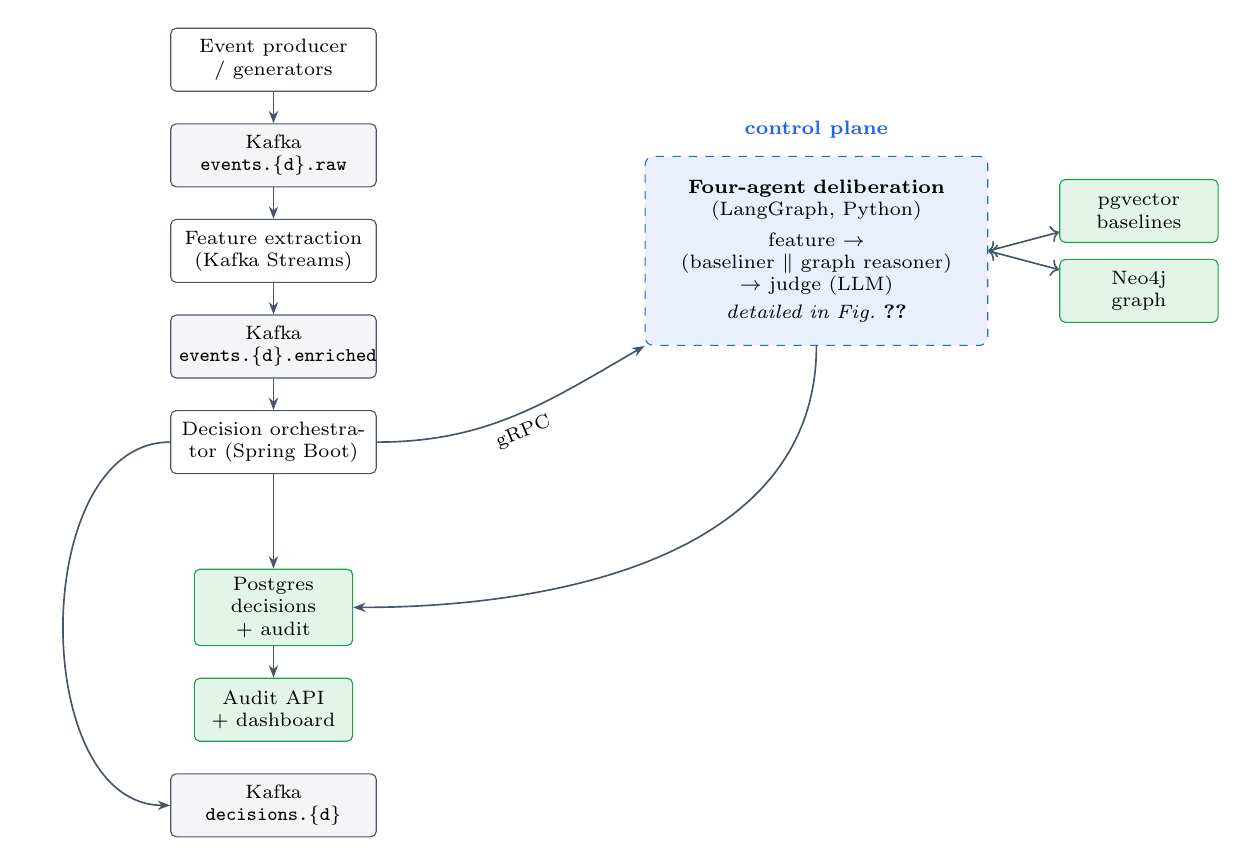
\begin{tikzpicture}[
  font=\scriptsize,
  box/.style={draw=cslate,rounded corners=2pt,align=center,inner sep=3pt,
              minimum height=8mm,fill=white,text width=24mm},
  infra/.style={box,fill=cgray!40,text width=24mm},
  store/.style={box,fill=cgreen!12,draw=cgreen,text width=18mm},
  delib/.style={draw=cblue,dashed,rounded corners=3pt,fill=cblue!10,
                align=center,inner sep=5pt,text width=40mm,minimum height=24mm},
  arr/.style={-{Stealth[length=4.5pt]},draw=cslate,semithick},
]
% ───────────────── DATA PLANE — vertical column, far left ─────────────────
\node[box] (prod) {Event producer / generators};
\node[infra,below=4mm of prod] (raw) {Kafka \texttt{events.\{d\}.raw}};
\node[box,below=4mm of raw] (stream) {Feature extraction (Kafka Streams)};
\node[infra,below=4mm of stream] (enr) {Kafka \texttt{events.\{d\}.enriched}};
\node[box,below=4mm of enr] (orch) {Decision orchestrator (Spring Boot)};
\node[store,below=12mm of orch] (pg) {Postgres\\decisions + audit};
\node[store,below=4mm of pg] (api) {Audit API\\+ dashboard};
\node[infra,below=4mm of api] (dec) {Kafka \texttt{decisions.\{d\}}};

\draw[arr] (prod) -- (raw);
\draw[arr] (raw) -- (stream);
\draw[arr] (stream) -- (enr);
\draw[arr] (enr) -- (orch);
\draw[arr] (orch) -- (pg);
\draw[arr] (pg) -- (api);
\draw[arr] (orch.west) to[out=180,in=180] (dec.west);  % re-emit decisions, down the left

% ─────────── DELIBERATION — single box (see Fig. 2 for the DAG) ───────────
\node[delib,right=34mm of stream] (delib)
  {\textbf{Four-agent deliberation}\\(LangGraph, Python)\\[3pt]
   feature $\rightarrow$\\(baseliner $\parallel$ graph reasoner)\\$\rightarrow$ judge (LLM)\\[2pt]
   {\scriptsize\itshape detailed in Fig.~\ref{fig:delib}}};
\node[cblue,font=\scriptsize\bfseries,above=1mm of delib] {control plane};

% ───────────────── STORES — right of the deliberation box ─────────────────
\node[store,above right=1mm and 9mm of delib.east] (pgv) {pgvector\\baselines};
\node[store,below right=1mm and 9mm of delib.east] (neo) {Neo4j\\graph};
\draw[arr,<->,cslate] (delib.east) -- (pgv);
\draw[arr,<->,cslate] (delib.east) -- (neo);

% ───────────────── CROSS-ZONE — gRPC in, decision out ─────────────────
\draw[arr] (orch.east) to[out=0,in=-150] node[below,font=\scriptsize,sloped]{gRPC} (delib.south west);
\draw[arr] (delib.south) to[out=-90,in=0] (pg.east);
\end{tikzpicture}
\caption{\textsc{Conclave} event lifecycle. The \emph{data plane} (Java/Spring
Boot, left) handles ingestion, Kafka Streams feature extraction, the decision
write path, and the audit API. The \emph{control plane} (Python/LangGraph, centre)
runs the four-agent deliberation behind a gRPC boundary; its two context agents
query the backing stores (right). The internal deliberation DAG is shown in
Figure~\ref{fig:delib}. Only feature extraction and the graph schema are
domain-specific.}
\label{fig:arch}
\end{figure*}

\subsection{The deliberation graph}

The deliberation itself is a small, fixed LangGraph DAG~\cite{langgraph2024}
(Figure~\ref{fig:delib}). The feature node runs first and produces a structured
digest. Two context nodes---the behavioral baseliner and the graph
reasoner---then run \emph{in parallel}; each has a strict budget of a single
gRPC call to its backing service and a per-call deadline. Their findings join,
and the judge node runs last. This shape is latency-optimal: the two slow-ish
context lookups overlap, and only the judge (the LLM call) is on the critical
path alone.

\begin{figure}[t]
\centering
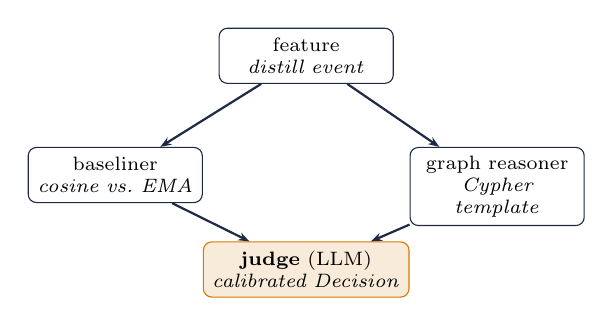
\begin{tikzpicture}[
  font=\scriptsize,
  node distance=6mm,
  n/.style={draw=cnavy,rounded corners=3pt,align=center,minimum height=7mm,
            fill=white,text width=20mm,inner sep=3pt},
  jn/.style={n,fill=camber!15,draw=camber,text width=24mm},
  arr/.style={-{Stealth[length=4pt]},draw=cnavy,thick},
]
\node[n] (feat) {feature\\\emph{distill event}};
\node[n,below left=8mm and 2mm of feat] (base) {baseliner\\\emph{cosine vs.\ EMA}};
\node[n,below right=8mm and 2mm of feat] (graph) {graph reasoner\\\emph{Cypher template}};
\node[jn,below=20mm of feat] (judge) {\textbf{judge} (LLM)\\\emph{calibrated Decision}};

\draw[arr] (feat) -- (base);
\draw[arr] (feat) -- (graph);
\draw[arr] (base) -- (judge);
\draw[arr] (graph) -- (judge);
\end{tikzpicture}
\caption{The deliberation DAG: \texttt{feature} $\rightarrow$ (\texttt{baseliner}
$\parallel$ \texttt{graph}) $\rightarrow$ \texttt{judge}. Any context node may
fail or time out; its branch contributes an error note and the judge proceeds on
the remaining evidence. If the judge itself is unavailable, a deterministic
fallback derives a safe verdict from the structured findings.}
\label{fig:delib}
\end{figure}

\subsection{The evidence package}

The judge never sees raw data; it sees a structured \emph{evidence package}:
(i) the feature digest (headline + bullets + numeric features carried through for
quantitative reasoning); (ii) the behavioral finding---cosine similarity to the
entity's rolling embedding, a derived anomaly score, and a cold-start flag for
entities with no history; and (iii) the graph finding---a \emph{named} template
result with a structural \texttt{risk\_signal} in $[0,1]$. Keeping the evidence
structured (rather than free text) lets every node be unit-tested and lets the
judge cite specific quantities.

\paragraph{Behavioral baseline (vectors, not statistics).}
Each entity carries a 384-dimensional ``fingerprint'': an exponential moving
average (EMA) of the embeddings of its past events, computed with a local
sentence-transformer~\cite{reimers2019sbert} and stored in
\texttt{pgvector}~\cite{pgvector}. A new event $e$ is embedded and scored by
cosine similarity to the entity's fingerprint $\mu$; the anomaly score is the
clipped, scaled cosine distance,
$a(e) = \min\!\big(1,\ \max(0,\ 1-\cos(e,\mu))/d_{\max}\big)$.
A naive high-decay EMA would pin a new entity near its very first event for many
updates; we ramp the effective decay, $\textit{eff} = \min(\textit{decay},\ 1 -
1/n)$ for event count $n$, so the profile behaves as a simple average for the
first $\approx 1/(1-\textit{decay})$ events and as a true EMA thereafter
(\textit{decay}$=0.85$ by default, $\approx$ a 7-event memory). Scoring is
strictly read-only: a suspicious event is compared against, but never folded
into, the profile it is measured against, so an attack cannot poison its own
baseline within a single decision.

\paragraph{Graph reasoner (named, bounded templates).}
Rather than generate Cypher with an LLM, the graph reasoner runs a fixed,
audited set of depth-bounded templates and returns \emph{named} findings the
judge can cite verbatim (e.g.\ \texttt{fraud\us card\us testing\us ring},
\texttt{security\us lateral\us movement}). Each template maps a structural count to a
monotone risk curve: the card-testing template fires once a single device fans
out across more than three cardholders; the lateral-movement template is silent
below five distinct hosts, ramps from $0.60$ at the five-host threshold, and
crosses $0.80$ (``confirmed'') as the fan-out widens, capped so the signal is
never inflated past what the count supports. Fixed templates trade recall on
novel structures for predictable latency (\S\ref{sec:eval}) and for the
explainability of a named pattern.

\subsection{Calibration and the judge contract}

The judge is instructed to output a typed \texttt{Decision}: a score in $[0,1]$,
a verdict label from the fixed band, an ordered list of contributing factors with
signed weights in $[-1,1]$, and a 2--4 sentence Markdown explanation. The
calibration philosophy is encoded in the system prompt and is the most important
design lever in the system: \emph{anchor the score on the strongest piece of
direct evidence---a severe rule indicator or a confirmed named graph
pattern---and treat the behavioral embedding as the weakest, most easily fooled
signal.} The prompt explicitly warns that when an attacker repeats a malicious
action, the entity's rolling profile drifts toward the attack, so cosine
similarity stays high (anomaly low) mid-attack; a ``normal'' embedding is weak
corroboration, never exoneration. This guidance is what lets the judge
\textsc{block} a card-testing ring even though the ring's behavior looks
self-consistent (Figure~\ref{fig:qual}).

\subsection{Graceful degradation}

The pipeline never returns ``no decision.'' Each context node catches its own
errors and degrades to an empty finding plus an error note; the parallel join
concatenates errors without clobbering successful siblings. If the judge LLM is
unavailable or returns an unparseable response, a deterministic fallback combines
the structured signals (graph risk, cold-start prior, behavioral anomaly) into a
safe, explainable verdict that leans toward \textsc{review} on ambiguity. In our
benchmark runs, zero of \fraudndec{}$+$\secndec{} decisions hit the dead-letter
queue.

\subsection{Key design decisions}

Several decisions follow from the goal of one architecture serving many domains
under a latency budget, and are worth stating explicitly because they shaped the
results in \S\ref{sec:eval}.

\begin{enumerate}
  \item \textbf{Java data plane, Python control plane.} The high-throughput
        Kafka consumer and the transactional decision-write path are Java; the
        stateful agent graph is Python/LangGraph. The gRPC seam keeps the
        ``Java = data, Python = reasoning'' separation legible and lets each side
        use its native ecosystem.
  \item \textbf{Three context agents in parallel, one judge after.}
        Latency-optimal: the two backing-service lookups overlap, leaving only
        the LLM round-trip on the critical path alone (Figure~\ref{fig:delib}).
  \item \textbf{Vectors over hand-built statistics for baselines.} A rolling
        per-entity embedding captures ``looks like this customer'' more flexibly
        than a fixed bank of velocity/z-score features---at the documented cost
        that it is blind to categorical attacks (\S\ref{sec:eval}).
  \item \textbf{Fixed Cypher templates, never LLM-generated queries.} Bounded
        depth gives predictable latency; \emph{named} findings give the judge
        something concrete to cite; an audited template set is reviewable.
  \item \textbf{A calibrated score, not a binary.} Downstream consumers
        (step-up auth, SOC triage) need a number; the verdict band is a view on
        the score, not a replacement for it.
  \item \textbf{Pluggable judge behind one parser.} The provider factory makes
        the judge a swappable component, decoupling the architecture from any
        single vendor and enabling a fully local (Ollama) deployment.
\end{enumerate}

%% ===========================================================================
\section{Implementation}
%% ===========================================================================

The data plane is Java~25 on Spring Boot~4.0 with Kafka Streams; the control
plane is Python~3.12 on LangGraph. They communicate over gRPC. This split is
deliberate: Java handles the high-throughput consumer and the transactional
write path, while Python hosts the stateful agent graph where LangGraph's
parallel fan-out and conditional edges are natural. The judge backend is chosen
at startup by an \texttt{LLMProvider} factory keyed on
\texttt{JUDGE\us LLM\us PROVIDER}: \texttt{anthropic} (Claude via tool-use structured
output, with prompt caching on the system block), \texttt{openai} (any
OpenAI-compatible endpoint---OpenAI, OpenRouter, Groq---via JSON mode), or
\texttt{ollama} (a local model via \texttt{format="json"}). All three share one
parser and one fallback, so the rest of the system is backend-agnostic. The
behavioral embeddings run in-process via a Java sentence-transformer, so the
\emph{only} remote dependency that varies is the judge.

\begin{table}[t]
\centering
\small
\caption{Implementation footprint. LOC excludes generated code (Avro, protobuf
stubs) and tests.}
\label{tab:loc}
\setlength{\tabcolsep}{4pt}
\begin{tabular}{@{}lrl@{}}
\toprule
Component & LOC & Stack \\
\midrule
Orchestrator & 2{,}819 & Spring Boot, Kafka \\
Baseline service & 1{,}051 & pgvector, MiniLM \\
Graph reasoner & 1{,}108 & Neo4j \\
Generators & 1{,}723 & Java \\
Deliberation agents & 2{,}183 & LangGraph, gRPC \\
Dashboard + site & 2{,}548 & React, Vite \\
\midrule
\multicolumn{3}{@{}l@{}}{Tests: 219 Java + 99 Python; CI gate $\ge$80\% line cov.} \\
\bottomrule
\end{tabular}
\end{table}

\paragraph{Domain configuration.} Switching domains sets one environment
variable (\texttt{SPRING\us PROFILES\us ACTIVE}). The same images then bind
fraud-specific or security-specific feature specs, Avro schemas, and graph
templates. No code is forked per domain; domain-specific logic lives only in the
feature extractors and the Cypher templates, as Table~\ref{tab:loc}'s shared
components make concrete. Table~\ref{tab:domains} makes the mapping explicit: the
two domains differ in their event type, entity, graph schema, and adversarial
patterns, but share the deliberation graph, the calibration band, the judge, the
decision schema, and the audit surface.

\begin{table}[t]
\centering
\caption{One architecture, two configurations. Everything below the rule is
shared verbatim; only the rows above it change per domain.}
\label{tab:domains}
\begin{tabular}{lll}
\toprule
 & \textbf{Payment fraud} & \textbf{Security / SOC} \\
\midrule
Event   & card-not-present txn   & auth / resource access \\
Entity  & cardholder / card      & principal / identity \\
Graph   & cardholder--device--IP & principal--host--resource \\
        & --merchant             & \\
Patterns& card-testing ring,     & lateral movement, \\
        & bust-out, ATO          & exfiltration, ATO \\
\midrule
\multicolumn{3}{l}{\emph{Shared:} deliberation DAG, evidence schema, EMA} \\
\multicolumn{3}{l}{baseliner, calibration band, judge, \texttt{Decision}} \\
\multicolumn{3}{l}{schema, audit API, dashboard, degradation path} \\
\bottomrule
\end{tabular}
\end{table}

%% ===========================================================================
\section{Evaluation}
\label{sec:eval}
%% ===========================================================================

\subsection{Methodology}

We evaluate end-to-end through the running stack---no offline re-scoring. The
synthetic generators emit a multi-day, multi-customer organic population (so that
per-entity baselines converge before any attack), then inject labeled adversarial
campaigns. Crucially, ground-truth labels are published to a \emph{separate} Kafka
topic (\texttt{events\dt\{domain\}\dt labels}) that the orchestrator never subscribes
to, so there is no label leakage into the decision path. Our harness reads the
persisted decisions from the audit API and joins them against the label topic on
\texttt{event\_id}.

The judge for these runs is \judgemodel{} served via \judgeendpoint{} (an
OpenAI-compatible endpoint). We report this configuration honestly: it is a
commodity, low-cost hosted model, not the project's canonical Claude Haiku
backend. Because the architecture is provider-agnostic, the numbers here
characterize \emph{this} judge; a stronger judge would be expected to do at least
as well. We use identical generator parameters across domains
(8 entities $\times$ 7 days $\times$ 3 events/day organic population; 40 extra
clean events; 2 ring/lateral, 2 ATO, 2 bust-out/exfiltration campaigns),
yielding \fraudndec{} fraud and \secndec{} security decisions.

Every number below comes from a clean run of the published stack---three commands
per domain (bring the stack up in serving mode, fire the labeled synthetic burst,
capture):

\begin{lstlisting}[style=decision]
./scripts/up.sh   serving fraud
./scripts/seed.sh fraud --customers 8 --days 7 \
  --events-per-day 3 --clean 40 --rings 2 --ato 2 --extra 2
python3 benchmark/capture.py --domain fraud --tag run
\end{lstlisting}

\noindent The harness pages the audit API for all decisions, drains the
ground-truth label topic from Kafka, joins on \texttt{event\_id}, and emits the
confusion matrices, ROC-AUC, per-attack-type recall, score separation, and
latency percentiles reported here. ROC-AUC uses the tie-aware Mann--Whitney
formulation; precision@FPR sweeps unique score thresholds. The generator is
seeded deterministically, so the event population is fixed; only the judge's LLM
responses vary run-to-run, and two independent runs reproduced the fraud AUC to
within $\pm0.0004$ (measured $0.9985$ and $0.9989$) at the same
zero-false-positive \textsc{block} operating point.

\subsection{Detection: fraud}

On the fraud configuration (Table~\ref{tab:detect}), \textsc{Conclave} attains
ROC-AUC \fraudauc{}. The score cleanly separates classes: clean events average
\fraudcleanmean{} while attacks average \fraudattackmean{}
(Figure~\ref{fig:hist}, top). At the \textsc{block} threshold ($\ge 0.70$),
precision is \fraudblockprec\% with \emph{zero} false positives
(\fraudblocktp{}~TP, \fraudblockfp{}~FP, \fraudblockfn{}~FN, \fraudblocktn{}~TN)
and recall \fraudblockrec\%. Widening the operating point to ``flagged''
(\textsc{block} \emph{or} \textsc{review}) raises recall to \fraudflagrec\%---%
\emph{every} attack is surfaced for a human---at \fraudflagprec\% precision and a
\fraudflagfpr\% false-positive rate. At a fixed FPR~$\le 1\%$ the score achieves
\fraudponeprec\% precision and \fraudponerec\% recall. Per attack type, all three fraud
campaigns---card-testing rings ($n{=}\fraudncardtestingring$), account-takeover
($n{=}\fraudnfraudato$), and bust-out ($n{=}\fraudnbustout$)---are flagged at
100\% recall at the review-or-higher operating point.

\subsection{Detection: security, and the evidence-coverage lesson}

The security configuration tells a more interesting story (Table~\ref{tab:detect},
lower block; Table~\ref{tab:pertype}). Overall AUC is \secauc{}, and the
\textsc{block} threshold again yields \secblockprec\% precision with zero false
positives---but recall is only \secblockrec\%. Breaking recall down by attack type
explains why:

\begin{itemize}
  \item \textbf{Lateral movement} ($n{=}\secnlateralmovement$): recall
        \secreclateralmovement\%. These attacks fan a single principal across many
        hosts, which the \texttt{security\us lateral\us movement} Cypher template
        detects directly; once the fan-out crosses the template's host threshold,
        the judge \textsc{block}s with score $0.95$ and cites the named pattern
        (Figure~\ref{fig:qual}, lower). The misses are early events in a campaign,
        \emph{before} enough hosts are touched for the structural signal to fire.
  \item \textbf{Exfiltration} ($n{=}\secnexfiltration$): recall
        \secrecexfiltration\%. Every exfiltration event scored $0.15$
        (\textsc{allow}).
  \item \textbf{Security account-takeover} ($n{=}\secnsecurityato$): recall
        \secrecsecurityato\%. Scores clustered at $0.05$--$0.15$ (\textsc{allow}).
\end{itemize}

The exfiltration and ATO misses are not random: they are a direct,
explainable consequence of \emph{evidence coverage}. Exfiltration in our
generator is a single principal reading many \emph{sensitive resources} in
sequence---a signal that a privileged-access template would surface, but the
security deliberation's hot path invokes only the lateral-movement template. With
no host fan-out and no privileged-access finding, the judge sees a successful
authentication, a ``normal'' embedding, and \emph{nothing structural to act on};
it correctly (given its inputs) returns \textsc{allow}. Security ATO is worse:
its discriminative signal is a behavioral break (geo, time-of-day, auth method)
that the same-entity embedding is, by the prompt's own admission, blind
to---when the attacker's events accumulate, the profile drifts toward them.

This is the paper's central lesson, and we state it plainly: \textbf{a
deliberation architecture is bounded by the evidence its agents compute. The
judge is a weigher of presented evidence, not an oracle; it cannot recover a
discriminative signal that no agent extracted.} The fix is not a better
prompt---it is wiring the privileged-access template into the security hot path
and adding a non-self-referential anomaly signal for ATO. We report the
un-patched numbers deliberately, because the failure mode is the finding.

\begin{table}[t]
\centering
\caption{End-to-end detection. ``Block'' is the verdict $\ge 0.70$ operating
point; ``Flagged'' is \textsc{block}-or-\textsc{review} ($\ge 0.30$). Judge:
\judgemodel.}
\label{tab:detect}
\begin{tabular}{llrrrr}
\toprule
Domain & Op.\ point & Prec.\ & Recall & FPR & AUC \\
\midrule
\multirow{2}{*}{Fraud (\fraudndec{})}
  & Block          & \fraudblockprec\% & \fraudblockrec\% & \fraudblockfpr\% & \multirow{2}{*}{\fraudauc} \\
  & Flagged        & \fraudflagprec\% & \fraudflagrec\% & \fraudflagfpr\% & \\
\midrule
\multirow{2}{*}{Security (\secndec{})}
  & Block          & \secblockprec\% & \secblockrec\% & \secblockfpr\% & \multirow{2}{*}{\secauc} \\
  & Flagged        & \secflagprec\% & \secflagrec\% & \secflagfpr\% & \\
\bottomrule
\end{tabular}
\end{table}

\begin{table}[t]
\centering
\caption{Per-attack-type recall at the flagged (review-or-higher) operating
point. Detection tracks evidence coverage: patterns with a dedicated agent signal
are caught; those without are missed.}
\label{tab:pertype}
\begin{tabular}{lllr}
\toprule
Domain & Attack type & Surfacing signal & Recall \\
\midrule
Fraud & Card-testing ring & graph template & \fraudreccardtestingring\% \\
Fraud & Account-takeover  & rule features  & \fraudrecfraudato\% \\
Fraud & Bust-out          & rule features  & \fraudrecbustout\% \\
\midrule
Security & Lateral movement & graph template & \secreclateralmovement\% \\
Security & Exfiltration     & \emph{none in hot path} & \secrecexfiltration\% \\
Security & Account-takeover & \emph{embedding blind} & \secrecsecurityato\% \\
\bottomrule
\end{tabular}
\end{table}

\begin{figure}[t]
\centering
% --- fraud histogram ---
\begin{tikzpicture}
\begin{axis}[
  width=\columnwidth,height=3.4cm,
  ybar stacked,bar width=5pt,
  ymin=0,enlarge x limits=0.06,
  xlabel={risk score},ylabel={\#events},
  xlabel style={font=\scriptsize},ylabel style={font=\scriptsize},
  tick label style={font=\tiny},
  title={\scriptsize Fraud: score distribution (clean vs.\ attack)},
  legend style={font=\tiny,at={(0.5,1.02)},anchor=south,legend columns=2,draw=none},
  xtick={0.05,0.25,0.45,0.65,0.85},
]
\addplot[fill=cgreen!55,draw=cgreen!70!black] table[x=center,y=clean] {data/fraud_hist.dat};
\addplot[fill=cred!60,draw=cred!70!black] table[x=center,y=attack] {data/fraud_hist.dat};
\legend{clean,attack}
\end{axis}
\end{tikzpicture}\\[2pt]
% --- security histogram ---
\begin{tikzpicture}
\begin{axis}[
  width=\columnwidth,height=3.4cm,
  ybar stacked,bar width=5pt,
  ymin=0,enlarge x limits=0.06,
  xlabel={risk score},ylabel={\#events},
  xlabel style={font=\scriptsize},ylabel style={font=\scriptsize},
  tick label style={font=\tiny},
  title={\scriptsize Security: score distribution (clean vs.\ attack)},
  xtick={0.05,0.25,0.45,0.65,0.85},
]
\addplot[fill=cgreen!55,draw=cgreen!70!black] table[x=center,y=clean] {data/security_hist.dat};
\addplot[fill=cred!60,draw=cred!70!black] table[x=center,y=attack] {data/security_hist.dat};
\end{axis}
\end{tikzpicture}
\caption{Calibrated-score histograms. In fraud (top) attacks concentrate near
$1.0$ and clean traffic near $0$, with almost no overlap (AUC \fraudauc). In
security (bottom) the caught attacks (lateral movement) sit at $0.95$ but a mass
of attacks (exfiltration/ATO) remains stuck in the low-score clean region---the
visual signature of the evidence-coverage gap (AUC \secauc).}
\label{fig:hist}
\end{figure}

\subsection{Latency}

End-to-end deliberation latency is dominated by the LLM judge. The two context
agents are fast and effectively free relative to the judge: the behavioral
lookup's measured p99 is $0.74$\,ms and the graph template's p99 is $6$\,ms on a
$\sim$100K-edge graph (component latency integration tests). The end-to-end
per-decision latency, including the hosted LLM round-trip, is summarized in
Table~\ref{tab:latency}: fraud p50 \fraudlatpfifty\,ms / p99 \fraudlatpninenine\,ms,
security p50 \seclatpfifty\,ms / p99 \seclatpninenine\,ms. The variance is the
hosted endpoint's, not the pipeline's---the deterministic stages contribute under
$10$\,ms combined. This locates the single optimization lever squarely at the
judge: model choice, prompt-cache hit rate, and batching.

\begin{table}[t]
\centering
\caption{End-to-end per-decision latency (ms), including the hosted judge
round-trip. Deterministic stages (baseline p99 $0.74$\,ms, graph p99 $6$\,ms)
are negligible; the judge dominates.}
\label{tab:latency}
\begin{tabular}{lrrrr}
\toprule
Domain & p50 & p95 & p99 & max \\
\midrule
Fraud    & \fraudlatpfifty & \fraudlatpninefive & \fraudlatpninenine & \fraudlatmax \\
Security & \seclatpfifty   & \seclatpninefive   & \seclatpninenine   & \seclatmax \\
\bottomrule
\end{tabular}
\end{table}

\subsection{Cross-domain transfer}

The headline domain-agnosticism claim holds at the architectural level: both
configurations run on the same binaries, the same deliberation graph, the same
calibration band, the same audit surface, and the same judge, differing only in
feature specs and graph templates. The fraud configuration demonstrates that when
the domain's discriminative patterns are wired as agent signals, the shared
architecture delivers production-grade detection (AUC \fraudauc, zero
false-positive blocks). The security configuration demonstrates the converse and
the boundary condition: the architecture transfers, but \emph{detection quality
transfers only as far as evidence coverage}.

\subsection{Qualitative output}

Figure~\ref{fig:qual} shows two real \texttt{Decision} records from the runs. The
fraud example \textsc{block}s a card-testing ring with a precise, analyst-actionable
rationale and signed contributing factors, including an explicit note that the
``normal'' behavioral signal is disregarded as an artifact of repetitive automated
testing---exactly the calibration discipline from \S\ref{sec:design}. The security
example shows the same reasoning pattern catching lateral movement. These are
verbatim outputs, not curated paraphrases.

\begin{figure}[t]
\begin{lstlisting}[style=decision]
// FRAUD -- card-testing ring, score 0.95 -> BLOCK
"verdict_explanation_md":
  "This transaction is part of a confirmed
   `fraud_card_testing_ring` involving 8 distinct
   cardholders sharing a single device. The graph
   reasoning signal is decisive (risk_signal=1.00),
   and the behavioral baseline's lack of anomaly is
   disregarded as it reflects the attacker's
   consistent, repetitive testing behavior.",
"contributing_factors": [
  {"name":"graph_ring_detected","weight":1.0, ...},
  {"name":"no_anomaly_observed","weight":-0.1, ...}]

// SECURITY -- lateral movement, score 0.95 -> BLOCK
"verdict_explanation_md":
  "The event is part of a confirmed
   `security_lateral_movement` graph pattern ...
   accessing 8 distinct hosts in a suspicious
   sequence. Despite the high cosine similarity,
   this behavioral signal is disregarded ... The
   graph evidence is decisive."
\end{lstlisting}
\caption{Verbatim judge outputs (abridged). Both domains share the same decision
shape and the same calibration discipline---anchor on the confirmed graph
pattern, discount the self-consistent embedding.}
\label{fig:qual}
\end{figure}

%% ===========================================================================
\section{Discussion and Limitations}
%% ===========================================================================

\paragraph{The judge is a bottleneck---of latency and of evidence.}
Two senses. Operationally, the LLM dominates latency (Table~\ref{tab:latency}),
so throughput scales with judge concurrency and cache hit rate, not with the data
plane. Epistemically, the judge is bounded by the evidence package; the security
result shows that no amount of judging recovers an un-extracted signal. Both point
to the same engineering priority: invest in \emph{agent coverage} and in judge
serving, in that order.

\paragraph{Calibration is empirical, not theoretical.}
The threshold band and the score anchoring are validated against labeled streams,
not derived from a calibration guarantee~\cite{guo2017calibration}. A different
judge model will shift the score distribution; the band would need
re-validation. We do not claim transferable calibration across judge backends.

\paragraph{Synthetic evaluation.}
Our adversarial streams are generated, not production traffic, so absolute
numbers should be read as characterizing the architecture under known, labeled
conditions---not as a claim about real-world IEEE-CIS~\cite{ieeecis2019} or
BETH~\cite{highnam2021beth} performance, which we leave to future work. The
generators do encode realistic structure (multi-day baselines, mixed amount
distributions, ring/lateral fan-out), and the leakage-proof label topic makes the
join trustworthy.

\paragraph{No comparison to a tuned GBT baseline.}
We deliberately do not claim to beat XGBoost on AUC; a well-tuned GBT will likely
win on raw discrimination. \textsc{Conclave}'s claim is architectural:
explainability by construction, domain-agnosticism, and graceful degradation, at
competitive detection \emph{when evidence coverage is complete}. A head-to-head on
public datasets is the natural next study.

\paragraph{Single-judge, single-tenant.}
The judge is one LLM call, not an ensemble or a debate; we found a single
well-prompted judge over good evidence sufficient and cheaper. The system is
single-tenant by design scope.

%% ===========================================================================
\section{Conclusion}
%% ===========================================================================

\textsc{Conclave} treats multi-agent deliberation as a first-class risk-decision
architecture: specialized agents assemble a structured, per-event evidence
package and a calibrated LLM judge issues an explainable verdict, with the same
code serving payment fraud and security through configuration alone. End-to-end,
the fraud configuration reaches AUC \fraudauc{} with zero false-positive blocks
and flags every injected attack; the security configuration cleanly catches
graph-structural attacks and---honestly---misses attacks whose signal no agent
surfaces. That asymmetry crystallizes the design principle we most want
practitioners to take away: \emph{deliberation quality is upper-bounded by
evidence coverage}. Future work is concrete and architecture-internal: wire the
remaining graph templates into the security hot path, add a non-self-referential
anomaly signal for account-takeover, validate on IEEE-CIS and BETH, and benchmark
against a tuned GBT baseline. The complete stack, generators, benchmark harness,
and the \LaTeX{} source of this paper are open-source at
\url{https://github.com/Abhishek-Aditya-bs/Conclave}.

\bibliographystyle{ACM-Reference-Format}
\bibliography{references}

\end{document}
